In this chapter, we compare the three event detection methods from various standpoints. We will compare the original method (``original''), its modification based on greedy optimization of a different cost function (``greedy'') and the method using clustering algorithm to group similar words together (``cluster'').

Most of these evaluations rate the quality of the detected events on the keyword level. We will be referring to the average number of keywords per event, which we provide in an overview in \autoref{tab:events-overview}.

We discarded trivial events only consisting of a single keyword.

\hspace{\fill}

\begin{minipage}{\linewidth}
\centering
\begin{tabular}{ l c c c }\toprule[1.5pt]
\bf Method 	 & \bf Events detected & \bf Keywords & \bf Keywords per event \\ \midrule
\bf Original & 217 & 451 & 2.08 \\
\bf Greedy   & 46 & 473 & 10.28 \\
\bf Cluster & 77 & 761 & 9.88 \\ \bottomrule[1.25pt]
\end {tabular}\par
\captionof{table}{Overview of the detected events} \label{tab:events-overview}
\end{minipage}

\hspace{\fill}

As we can see from the table, the original method's events are not very rich, majority of them consisting of only 2 keywords. Since the original method is applied to the same words as the other methods detecting fewer events, we can expect a considerable level of redundancy, as we will see in \autoref{sec:redundancy}.

Furthermore, the keywords are used to query the document collection for event documents. Having only a few keywords makes it difficult to unambiguously retrieve related documents, leading to a poor document set. This will become clear in \autoref{sec:purity}.

The other two methods detect considerably fewer events which generally consist of a higher number of keywords. We can expect these methods to rank higher in the evaluations, provided that the events themselves are meaningful and not comprising of noisy words. This is an issue we will address in \autoref{sec:noise-evaluation}.

\section{Precision, Recall, F-measure}

First, we evaluate precision and recall with respect to a list of real events which occurred during the examined period. The list can be found in \autoref{app:real-events}.

We manually inspected the detected events and matched them with real world events. Out of this assignment, we calculated the precision, recall and F-measure. The results are shown in the table below.

\hspace{\fill}

\begin{minipage}{\linewidth}
\centering
\begin{tabular}{ l c c c }\toprule[1.5pt]
\bf Method 	 & \bf Precision & \bf Recall & \bf F-measure \\ \midrule
\bf Original &  16.35\%     & \bf 28.57\%     &  20.80\% \\
\bf Greedy   &  8.70\%     & 10.20\%      &  9.39\% \\
\bf Cluster &  \bf 25.97\%     & \bf 28.57\%      & \bf 27.21\% \\ \bottomrule[1.25pt]
\end {tabular}\par
\captionof{table}{Precision, Recall and F-measure comparison (manual evaluation)} \label{tab:title}
\end{minipage}

\hspace{\fill}

The original method's precision was poor due to high recurrence of events not appearing in the reference list, which will be more clear in redundancy evaluation later. As the average number of keywords per event is low, the real events are scattered among many detected events. On the other hand, the cluster-based method attained the highest precision due to events consisting of more keywords, meaning lower recurrence.

The greedy method's precision and recall were poor both for the same reason as the original method, as well as some events consisting of keywords unrelated to each other. This made them difficult to assign to their real world counterparts.\\

We also attempted to measure precision and recall in a more automatic way, so that the evaluation does not entirely depend on a manual input.

A real event, consisting of occurrence date and a headline, was considered detected if its date was found within a bursty period of some detected event, and if its headline had nonzero intersection with the detected event's keyword set.

\hspace{\fill}

\begin{minipage}{\linewidth}
\centering
\begin{tabular}{ l c c c }\toprule[1.5pt]
\bf Method 	 & \bf Precision & \bf Recall & \bf F-measure \\ \midrule
\bf Original &  7.14\%     & 16.33\%     &  9.94\% \\
\bf Greedy   &  \bf 26.09\%     & 22.45\%      &  \bf 24.13\% \\
\bf Cluster &  20.78\%     & \bf 28.57\%      &  24.06\% \\ \bottomrule[1.25pt]
\end {tabular}\par
\captionof{table}{Precision, Recall and F-measure comparison (automatic evaluation)} \label{tab:title} 
\end{minipage}

\hspace{\fill}

This method of evaluation favors the greedy approach whose keyword sets are richer and less coherent. This allows to intersect a headline more often due to seemingly random words appearing among the keywords.

On the other hand, the original method's keyword sets usually consist of only two words that may not appear in the headlines at all.

The cluster-based method's results are similar to the manual evaluation.

\section{Redundancy} \label{sec:redundancy}

Next, we evaluate redundancy --- the tendency to scatter a real event among several detected events. We manually collected occurrences of the same real event into groups, and computed the redundancy as $1 - (\left| \text{groups} \right| / \left| \text{events} \right|)$.

If it was unclear which real event does a detected event refer to, we considered it to be equal to some other event if they had similar burst characteristics and semantically similar keywords.

\hspace{\fill}

\begin{minipage}{\linewidth}
\centering
\begin{tabular}{ l c }\toprule[1.5pt]
\bf Method 	 & \bf Redundancy \\ \midrule
\bf Original &  77.99\% \\
\bf Greedy   &  65.22\% \\
\bf Cluster &  \bf 42.86\% \\ \bottomrule[1.25pt]
\end {tabular}\par
\captionof{table}{Redundancy comparison} \label{tab:title} 
\end{minipage}

\hspace{\fill}

Large redundancy of the original method is to be expected with events consisting of only 2 keywords on average.

\section{Noisiness} \label{sec:noise-evaluation}

When we checked the detected events manually, we noticed that some events are formed of keywords unrelated to each other, or do not show any clear bursts in their trajectory. Outputting such events is clearly undesirable, as they are difficult to make sense of.

Motivated by this, we seeked to evaluate the methods in terms of how many events they output share such noisy characteristic. We manually examined the events detected for signs of noise in trajectories or keyword sets. An event is considered noisy if its trajectory does not contain any distinguishable burst of activity, or if it consists of keywords unrelated of each other.

We realize that this examination is largely subjective. However, we did not find any simple way of automating the evaluation without losing interpretability of the results. It would be possible to impose a threshold on the overall event trajectory variance or keyword similarity, under which the event would be considered noisy. Such threshold would be an arbitrary value though, and the method could misclassify some events.

In \autoref{fig:noisy-event}, we show a typical noisy event that comes from the greedy algorithm. Not only are the keywords mostly unrelated to each other, they also do not carry much information about what real event could possibly be happening. The event trajectory does not contain many notable bursts. Perhaps except around day 290, the overall trajectory value does not vary greatly to reveal any burst of interest.

Although the keyword trajectories are not all similar, there could be an overlap high enough for them to be put together. We suspect that the main level of similarity comes from the Word2Vec model, though. It is well possible that these words appeared in similar context, even though they are not representative of any real event. The Word2Vec model would then rate them similar, and they would end up in one event.


\begin{figure}
\centering
\begin{subfigure}{.5\textwidth}
  \centering
  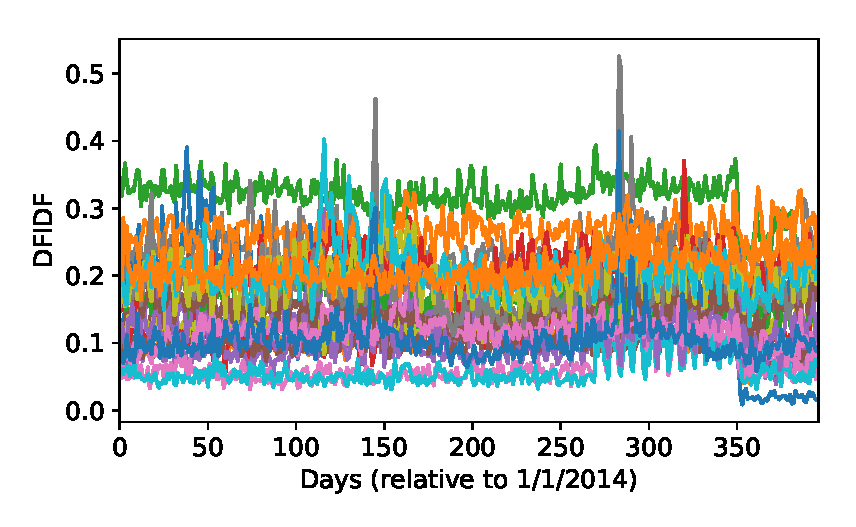
\includegraphics[width=\linewidth]{12_words}  % noisy keywords
  \caption{Event keyword trajectories}
  \label{fig:noisy-keywords}
\end{subfigure}%
\begin{subfigure}{.5\textwidth}
  \centering
  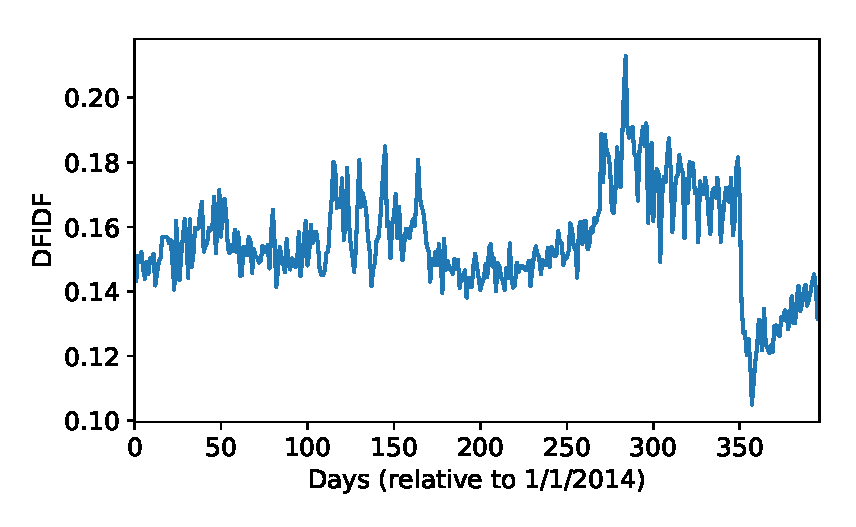
\includegraphics[width=\linewidth]{12_trajectory}  % noisy trajectory
  \caption{Trajectory of the same event}
  \label{fig:noisy-trajectory}
\end{subfigure}
\caption{(a) Event with noisy keywords and trajectory. The keywords are \textit{top, autor (author), podnik (business), test, fotogalerie (photogallery), reklama (advertisement), výsledek (result), komentář (commentary), zpravodajství (reporting), hra (game), informace (information), novinka (hot news), akce (action), návrh (proposition), Martin, klíčový (key, adj.), vedení (leadership), projekt (project), program, účast (participation), ČTK (Czech News Agency)}. (b) Trajectory of the same event constructed from the keywords.}
\end{figure} \label{fig:noisy-event}


\hspace{\fill}

\begin{minipage}{\linewidth}
\centering
\begin{tabular}{ l c }\toprule[1.5pt]
\bf Method 	 & \bf Noisiness \\ \midrule
\bf Original &  50.94\% \\
\bf Greedy   &  19.57\% \\
\bf Cluster &  \bf 19.48\% \\ \bottomrule[1.25pt]
\end {tabular}\par
\captionof{table}{Noisiness comparison} \label{tab:title} 
\end{minipage}

\hspace{\fill}

Here, the cluster-based method performed the best, as the clustering algorithm chosen (DBSCAN) is capable of automatic filtering of noisy samples. With the distance function measuring both trajectory and keyword similarity, it filters out words unrelated to any event.

Surprisingly, the greedy method performed only slighly worse than the cluster-based method. Although the greedy method reached considerable redundancy, manual check revealed that the events mostly consist of important keywords, and most of the trajectories contain distinguiushable bursts.

Poor performance of the original method is partially caused by its large redundancy. Even if a number of words with noisy trajectories appears in similar documents, the method would not group them together to a single event, but split into several noisy events. All of these noisy events then negatively contribute to the noisiness score.

\section{Purity} \label{sec:purity}

All previous evaluations concerned the events on the keyword level. The purity measure will evaluate the event document sets in terms of topical consistency. This is a metric used by \cite{document-purity} and the definition can be found in \cite{information-retrieval}.

The evaluation is an application of the standard measure of cluster purity in the sense that we measure the consistency of class labelling within each cluster. Each event is interpreted as a cluster of documents. Clearly, a high quality event should contain documents concerning similar topics. The problem is that our documents do not have any notion of class labels denoting their topics, which we will have to supplement.

Similarly to \cite{document-purity}, we first assembled a list of 50 words from 1000 most often occurring Nouns and Verbs in document headlines. The words are \textit{Ukrajina (Ukraine), Rusko (Russia), policie (police), soud (court), Zeman, EU, Sparta, festival, Babiš, Putin, Google, ekonomika (economics), letadlo (airplane), východ (east), politika (politics), zabít (to kill), poslanec (deputy), armáda (army), Kyjev (Kiev), Škoda, hokejista (hockey player), fotbalista (football player), doprava (traffic), vražda (murder), Vánoce (Christmas), Francie (France), sport, NATO, Moskva (Moscow), ropa (petroleum), turnaj (tournament), Obama, referendum, ebola, parlament (parliament), koalice (coalition), Paříž (Paris), automobil, mistrovství (championship), elektrárna (power plant), Sýrie (Syria), islamista (islamist), Brusel (Brussels), olympiáda (olympics), sníh (snow), průmysl (industry), revoluce (revolution), výbuch (explosion), finance, terorista (terrorist)}. All documents that contained any of these words in their headline were tagged with the corresponding class label.

Then, for each event, we computed the number of documents tagged by the most frequent label in the event. These values are then summed over all events and divided by the total number of tagged documents from all events.

Mathematically, this is formulated as

\begin{equation}
	\text{Purity} = \frac{1}{\left| \text{Tagged} \right|} \sum_{e \in \text{Events}}{\max_{t \in \text{Tags}} {\left| \{ d \in \doc{e} \mid d.\mathit{tag} = t \} \right|} },
\end{equation}

where $\text{Tagged} = \bigcup_{e \in \text{Events}}{\{ d \in \doc{e} \mid d.\mathit{tag} \text{ is defined} \}}$ and $\text{Tags}$ is a set containing the 50 manually selected words. The results are shown in \autoref{tab:purity}.

\hspace{\fill}

\begin{minipage}{\linewidth}
\centering
\begin{tabular}{ l c }\toprule[1.5pt]
\bf Method 	 & \bf Purity \\ \midrule
\bf Original &  30.53\% \\
\bf Greedy   &  44.42\% \\
\bf Cluster &  \bf 61.08\% \\ \bottomrule[1.25pt]
\end {tabular}\par
\captionof{table}{Purity comparison} \label{tab:purity} 
\end{minipage}

\hspace{\fill}

Poor performance of the original method can be explained by the events consisting mostly of 2 keywords. Such short query for the document collection does not distinguish the documents very well, often retrieving unrelated texts.

The other two methods yield events generally containing more keywords, so the queries are more specific. This allowed the Word Mover's Distance to retrieve more related documents.

\section{Computation time}

Finally, we evaluate the computation time. We measure the execution time of the individual detection steps, so it is clear which parts are the bottlenecks. All experiments were performed on a laptop computer with a 64bit operating system, quad-core processor and 8GB RAM.

In the greedy and cluster-based methods, we did not retrieve documents for periodic events with a period of 7 days or lower. The reason is that such short periods will essentialy cover the entire stream with short bursts and the Word Mover's Distance, computationally expensive on its own, will need to be computed to almost all documents. This might take a day's worth of time, and the short period events mostly concern unineresting events such as sport matches, weather forecasts, etc.

In addition, the summaries were extracted only using 50 most relevant documents, so that the overall process would not take too long.

\hspace{\fill}

\begin{minipage}{\linewidth}
\centering
\begin{tabular}{ r c c c }\toprule[1.5pt]
\bf Unit & \bf Original & \bf Greedy & \bf Clusters \\ \midrule
Word2Vec embedding & --- & \multicolumn{2}{c}{3h 50min} \\
Bag of words model construction & \multicolumn{3}{c}{37min} \\
Word trajectories \& spectral analysis & \multicolumn{3}{c}{8s} \\
Event detection & 2min 12s & 38s & 4min 50s \\
Document retrieval & 7min 30s & 6h & 7h 40min \\
Event annotation & 3h 13min & 8min 20s & 7min 30s \\ \midrule
\bf Total & 4h & 10h 36min & 12h 20min\\ \bottomrule[1.25pt]

\end{tabular}\par
\captionof{table}{Computation time comparison} \label{tab:title}
\end{minipage}

\hspace{\fill}

The original method's document retrieval took considerably less time than the other two methods. The reason is that the original method does not use the Word Mover's Distance as a similarity measure. Due to word semantic similarity being measured only in terms of their document overlap, there is always at least one document containing all the event keywords. It is sufficient to take the documents containing either of the event keywords and intersect these sets, which is much faster than calculating the distance.

This is also the reason why the event annotation took longer in the original method. Having also retrieved documents for events with short period (7 days and less), it is necessary to summarize each period independently. When we summarized only aperiodic events and those with period higher than 7 days, summarization took 1h 12min.

